\documentclass{beamer}
\author{Julius Elinson}
\usetheme{Frankfurt}
\usecolortheme{beaver}
\usepackage{multicol, amsmath,mathpazo}

\titlegraphic{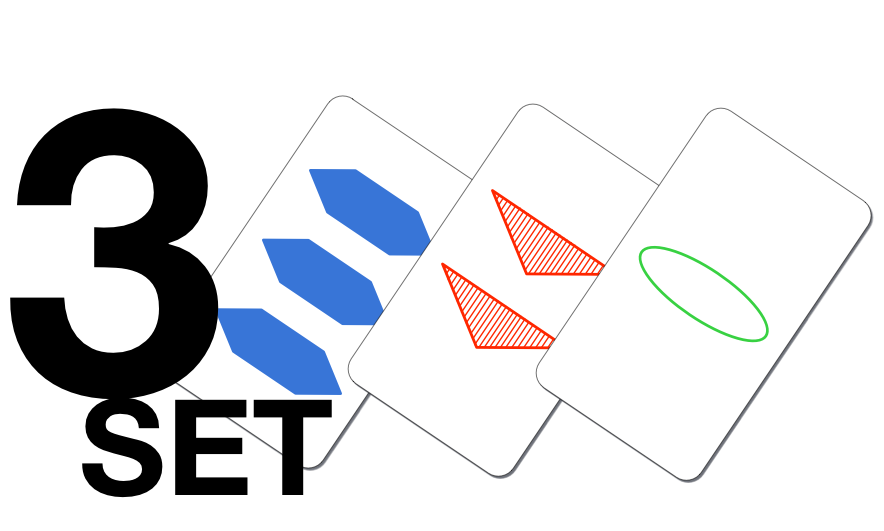
\includegraphics[width=.35\paperwidth]{img/logo.png}}

\title{3Set}
\subtitle{An iOS Game of Mixing \& Matching}
\institute{Aquincum Institute of Technology\\Harvey Mudd College}
\logo{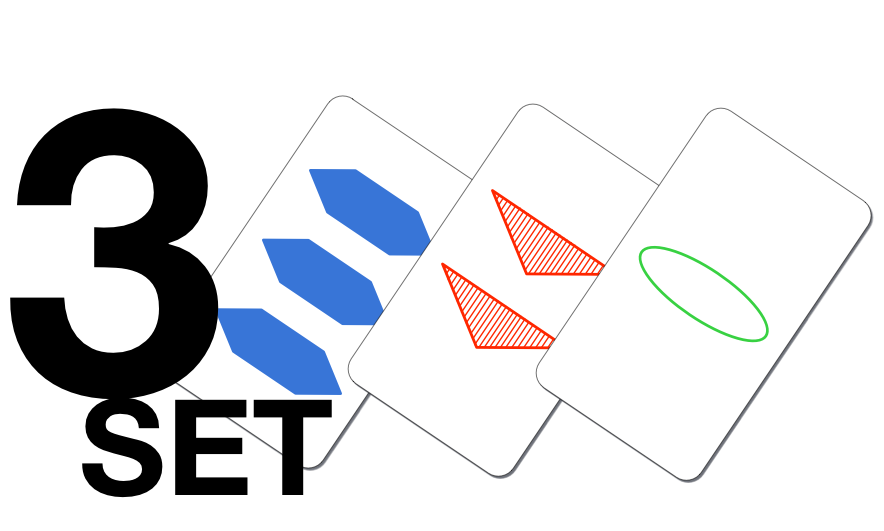
\includegraphics[width=.15\paperwidth]{img/logo.png}}

\beamertemplatenavigationsymbolsempty

\begin{document}
{
\setbeamertemplate{logo}{}
\begin{frame}
\maketitle
\end{frame}
}


\section{The Game}
\begin{frame}{Rock Climbing}
\begin{columns}

\begin{column}[T]{.5\linewidth}
%\includegraphics[height=\linewidth,angle=-90]{img/test2.JPG}
\end{column}
\pause
\begin{column}[T]{.6\linewidth}
\vspace{.8cm}
Problem Definition
\begin{itemize}
 \item Routes are color-delimited
 \item Use any subset of designated grips to get to the top
 \item Difficulty determined by size, spacing and surface properties of the grips
 \item Climbers have to determine a path
\end{itemize}

\end{column}

\end{columns}
\end{frame}

\begin{frame}[t]{Solution Specifications}
Input:
\begin{itemize}
 \item A low-resolution color photo of a rock wall
 \item Single pixel selection by user that maps to one of the grips in the desired route
\end{itemize}
\vspace{.3cm}
\pause

Output:
\begin{itemize}
 \item A viable path that minimizes a specified cost function
 \item Rendering of climber positions along the solution path
 \item Strain analysis
\end{itemize}

\pause
\vspace{.3cm}
Tools:
\begin{itemize}
 \item OpenCV Library
 \item Qt C++ Framework
\end{itemize}
\end{frame}

\section{Specifications}
\begin{frame}
 
\end{frame}

\section{Demo}
\begin{frame}
 
\end{frame}

\section{Implementation}
\begin{frame}
 
\end{frame}

\section{Future Work}
\begin{frame}
 
\end{frame}


\end{document}